% !TeX root = ../main.tex

\chapter{模型建構}

本章為模型建構,在介紹完研究過程中所會使用到的理論與方法後,需要將這些理論與方法根據應用情境建立模型並實際用於計算。在這一章節中,將闡述風速預測部分的時間序列預測模型建構流程,以及收益分析部分的風力電場與電動汽車等效模型,並於下一章節中將模型實際應用於案例中進行分析。

\section{風力電場發電預測}

\subsection{時間序列預測建模流程}

自迴歸移動平均模型 $\text{ARIMA}(p, d, q)$ 的建構流程如圖 \ref{figure: Time Series Model Flow} 所示。在取得時間序列資料後,需要先進行平穩性檢驗,若時間序列不具備平穩性則必須差分 $d$ 次進行平穩化;接著繪製其 ACF 與 PACF 圖形並由其特徵初步決定其自迴歸項 $p$ 與移動平均項 $q$ 之值;初步階數選定之後透過 AIC 與 BIC 進行評價並選出最適模型以進行時間序列預測。

\begin{figure}[htbp]
  \centering
  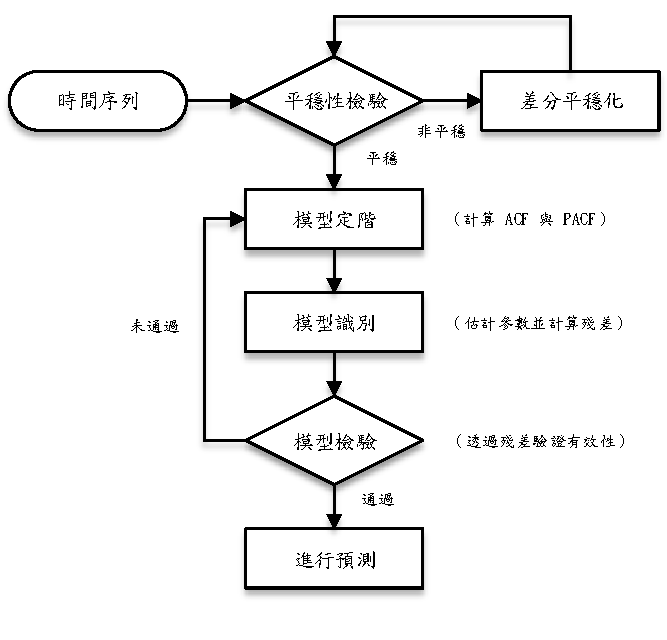
\includegraphics{time_series_model_flow}
  \caption{時間序列預測建模流程}
  \label{figure: Time Series Model Flow}
\end{figure}

\subsection{支持向量迴歸建模流程}

支持向量迴歸模型的建構流程如圖 \ref{figure: Support Vector Regression Flow} 所示,在取得資料之後,會先將資料拆分為訓練集合 (training set) 與測試集合 (testing set),並選擇適當的核函數與特徵參數進行模型訓練,在計算出表現最佳的模型參數後,使用測試集合進行評價並選出最適模型進行預測。

\begin{figure}[htbp]
  \centering
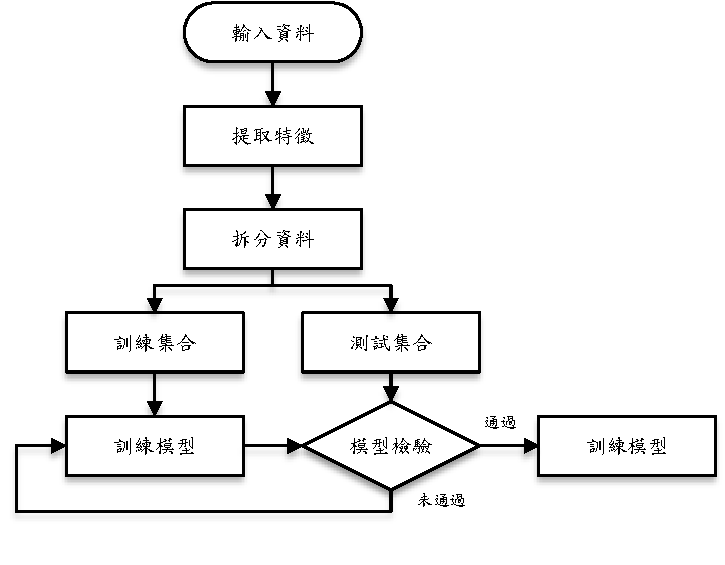
\includegraphics{support_vector_regression_model_flow}
  \caption{支持向量迴歸建模流程}
  \label{figure: Support Vector Regression Flow}
\end{figure}

\subsection{組合預測模型建模流程}

常見的組合預測模型是將預測的結果進行線性組合,根據加權方式可以再分為採用權重相等的簡單平均組合以及依據情境調整權重的變動權重組合,前者雖簡潔較易於計算但無法有效突出不同模型的優勢,後者則需要嘗試不同組合來尋找最佳的權重分配;本研究擬採用小波分解將原始時間序列進行解構,根據分解後各分量的特性分別採取較佳的預測方法後再將結果進行組合,組合時不需進行權重的分配。本研究將採用下述兩種組合預測模型,並比較其預測能力:
%
\begin{itemize}
  \item \textbf{一般等權組合預測模型} \\
        \begin{equation}\label{equation: Normal Combine Model}
          \hat{y}(t) = \frac{1}{2} \hat{y}_{\text{ARIMA}} (t) + \frac{1}{2} \hat{y}_{\text{SVR}} (t)
        \end{equation}
  \item \textbf{小波分解組合預測模型} \\
        \begin{equation}\label{equation: Wavelet Combine Model}
          \hat{y}(t) = \hat{A}_{2} (t) + \hat{D}_{1} (t) + \hat{D}_{2} (t)
        \end{equation}
\end{itemize}
%
上述模型的建構流程分別如圖 \ref{figure: Linear Combine Model Flow} 和圖 \ref{figure: Wavelet Combine Model Flow} 所示。一般等權組合預測模型即為分別使用單一預測模型進行預測後,將預測結果使用同樣的權重進行線性組合;小波分解組合預測模型則是將時間序列,透過離散小波轉換分解為近似分量與細節分量,並分別採用 ARIMA 模型與 SVR 模型進行預測,再將預測結果進行整合。

\begin{figure}[htbp]
  \centering
  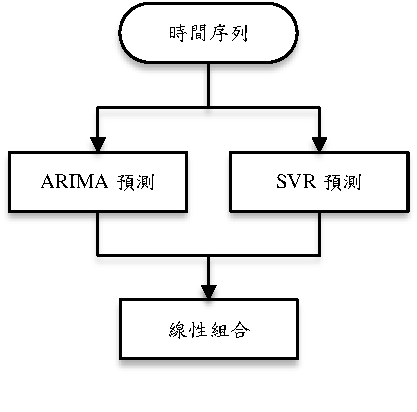
\includegraphics{linear_combine_model_flow}
  \caption[一般等權組合預測模型建模流程]{一般等權組合預測模型建模流程}
  \label{figure: Linear Combine Model Flow}
\end{figure}

\begin{figure}[htbp]
  \centering
  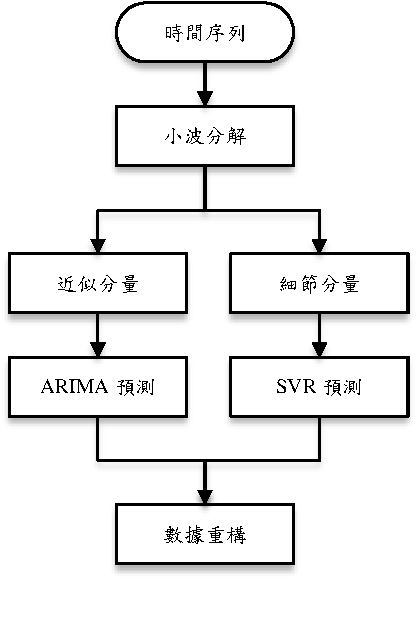
\includegraphics{wavelet_combine_model_flow}
  \caption[小波分解組合預測模型建模流程]{小波分解組合預測模型建模流程}
  \label{figure: Wavelet Combine Model Flow}
\end{figure}

\section{虛擬電廠收益分析}

\subsection{虛擬電廠架構概述}

本文採用的虛擬電廠 (Virtual Power Plant, VPP) 架構如圖 \ref{figure: Virtual Power Plant Model} 所示,由風力電場 (Wind Farm, WF)、電動汽車 (Electric Vehicle, EV) 組成,分別透過發電與儲能來參與電力市場 (Electric Market, EM)。

\begin{figure}[htbp]
  \centering
  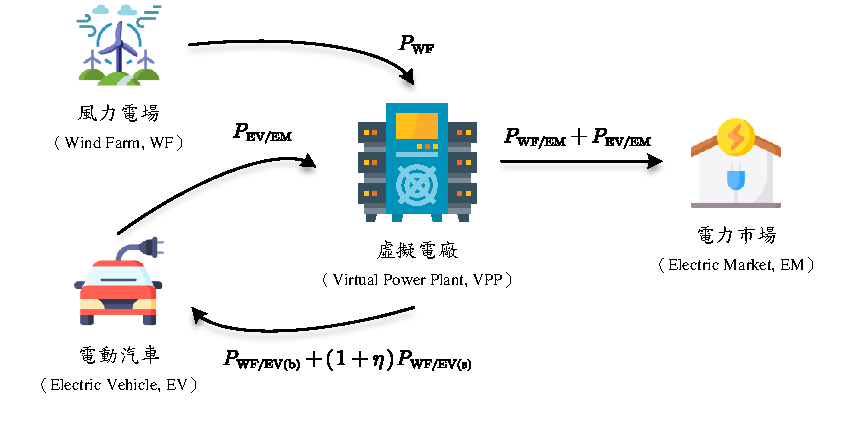
\includegraphics{virtual_power_plant_model}
  \caption{整合風力電場與電動汽車的虛擬電廠模型}
  \label{figure: Virtual Power Plant Model}
\end{figure}

由於風力電場發電數量預測仰賴於短期風速之預測結果,本研究考慮虛擬電廠參與日前市場交易之情境:在日前市場中,電網營運業者會在調度能源的前一天,提交電力需求並在競價後與發電業者簽署合約,規定發電業者提供約定的發電數量,如果與合約中保證的發電數量存在偏差則需要予以賠償;因此虛擬電廠作為發電業者,必須在第 $(t-1)$ 日提交價格資訊,並保證在第 $t$ 日的每個時段提供一定的發電數量。

對於虛擬電廠中的風力電場而言,需要在第 $(t-1)$ 日根據歷史風速資訊預測第 $t$ 日的風速,評估發電數量後給出在第 $t$ 日願意參與虛擬電廠的電動汽車數量與決定所需的最佳儲存數量,以此在日前市場中提出最有利的競標價格,並在滿足合約內容的前提下,根據實際的發電數量滾動式地持續更新其供應計畫。

對於虛擬電廠中的電動汽車而言,由於參與儲能後會增加電動汽車電池的充電放電次數,進而導致電池壽命減少,因此需要對電動汽車車主進行補償,以增加其參與虛擬電廠的意願。考量參與虛擬電廠的電動汽車無法如傳統儲能設備那般直接計算運轉成本,在本研究中不採用直接給予金錢的補償支付,而是無償地向電動汽車提供充電額度,亦即利用批發電價與零售電價之間差額的所得營收,換取電動汽車作為儲能設備的動機。

\subsection{風力電場等效模型}

若已知特定風力機組 $M$ 的額定功率曲線,則可以透過某一時段 $t$ 的風速資料 $v(t)$ 確定該時段所對應的風力機組發電狀況,如方程式 \eqref{equation: Wine Turbine Power} 所示。
%
\begin{equation}\label{equation: Wine Turbine Power}
  P_{\text{wt},M} (t) = P_{\text{wt},M} (v (t))
\end{equation}
%
假定一風力電場 (Wind Farm) 內設置有風力發電機組 $M_{1}, M_{2}, \dots, M_{k}$,則在當天某一時段 $t$ 的預測發電總量可以表示如方程式 \eqref{equation: Wind Farm Power} 所示。
%
\begin{equation}\label{equation: Wind Farm Power}
  P_{\text{WF}}(t) = \sum_{i = 1}^{k} P_{\text{wt}, M_i} (t)
\end{equation}
% %
% 在本文的模擬情況中,預測風速資料將以每一小時作為時間間隔,為了方便進行運算,最終將以向量形式表示在時間範圍內該風力電場不同單位時段的預測發電總量,用以參與電力市場作為日前市場的投標資訊,如方程式 \eqref{equation: Wind Farm Power Vector} 所示。
% %
% \begin{equation}\label{equation: Wind Farm Power Vector}
%   \boldsymbol{P_{\text{WF}}} = [ P_{\text{WF}}(1) P_{\text{WF}}(2) P_{\text{WF}}(3) \cdots P_{\text{WF}}(N) ]^{\top}
% \end{equation}

\subsection{電動汽車等效模型}

電動汽車透過儲存電能到電池中來參與虛擬電廠的電力市場交易,對於每一輛電動汽車 $V$ 而言都有其對應的儲存容量,假定一電動汽車 (Electric Vehicle) 集合中設置有電動汽車 $V_{1}, V_{2}, \dots, V_{h}$,則在當天某一時段 $t$ 的儲存容量上限可以表示如方程式 \eqref{equation: Electriv Vehicle Set Power} 所示。
%
\begin{equation}\label{equation: Electriv Vehicle Set Power}
  S_{\text{EV}}(t) = \sum_{i = 1}^{h} S_{V_i} (t)
\end{equation}
% %
% 在本文的模擬情況中,為配合以每一小時作為時間間隔的預測風速資料進行建模運算,同樣將以向量形式表示在時間範圍內,所有電動汽車在不同單位時段的儲存容量上限,如方程式 \eqref{equation: Electric Vehicle Power Vector} 所示。
% %
% \begin{equation}\label{equation: Electric Vehicle Power Vector}
%   \boldsymbol{S_{\text{EV}}} = [ S_{\text{EV}}(1) S_{\text{EV}}(2) S_{\text{EV}}(3) \cdots S_{\text{EV}}(N) ]^{\top}
% \end{equation}

\subsection{電力市場收益模型}

\subsubsection{日前市場調度}

根據前述架構,虛擬電廠將根據風力電場的預測發電數量,調度電動汽車進行儲存能量來參與電力市場交易,並透過規劃求解計算虛擬電廠的最大收益,其最佳化模型可由方程式 \eqref{equation: Virual Power Plant Profit Model} 表示。
%
\begin{subequations}\label{equation: Virual Power Plant Profit Model}
  \begin{alignat}{2}
    \max        \qquad & \sum_{t = 1}^{N} p_{e}(t) \times [P_{\text{WF/EM}}(t) + P_{\text{EV/EM}}(t)] \label{subequation: Virual Power Plant Profit Model 1} \\
    \text{s.t.} \qquad & P_{\text{WF/EM}}(t) + P_{\text{WF/EV(b)}}(t) + (1 + \eta)P_{\text{WF/EV(s)}}(t) = P_{\text{WF}}(t) \label{subequation: Virual Power Plant Profit Model 2} \\
                       & \sum_{i=1}^{t-1} \left[ P_{\text{WF/EV(s)}}(i) - P_{\text{EV/EM}}(i) \right] + P_{\text{WF/EV(s)}}(t) \leq P_{\text{ST}}(t) \label{subequation: Virual Power Plant Profit Model 3} \\
                       & \sum_{i=1}^{t-1} \left[ P_{\text{WF/EV(s)}}(i) - P_{\text{EV/EM}}(i) \right] - P_{\text{EV/EM}}(t) \geq 0 \label{subequation: Virual Power Plant Profit Model 4} \\
                       & P_{\text{WF/EV(b)}}(t) \geq \sigma P_{\text{ST}}(t) \label{subequation: Virual Power Plant Profit Model 5} \\
                       & 0 \leq P_{\text{ST}}(t) + P_{\text{WF/EV(b)}}(t) \leq S_{\text{EV}}(t) \label{subequation: Virual Power Plant Profit Model 6} \\
                       & P_{\text{WF/EM}}(t), P_{\text{WF/EV(s)}}(t),  P_{\text{WF/EV(b)}}(t),P_{\text{EV/EM}}(t) \geq 0 \label{subequation: Virual Power Plant Profit Model 7}
  \end{alignat}
\end{subequations}
%
其中,$p_{e} (t)$ 為虛擬電廠在電力交易市場中的販售電力價格;$P_{\text{WF/EM}}(t)$ 為風力電場輸送至電力交易市場中進行販售的電力數量;$P_{\text{WF/EV(s)}}(t)$ 為風力電場輸送至電動汽車電池中進行儲存的電力數量;$P_{\text{WF/EV(b)}}(t)$ 為風力電場輸送至電動汽車電池中作為補償的電力數量;$P_{\text{EV/EM}}(t)$ 為電動汽車輸送至電力交易市場中進行販售的電力數量;$P_{\text{ST}}(t)$ 為虛擬電廠需要的電力儲存容量;$\eta$ 為電動汽車電池在充放電過程的能量轉換損耗比例 ($\eta \in [0, 1]$)。

% 目標函數說明
式 \eqref{subequation: Virual Power Plant Profit Model 1} 為目標函數,為了使得電動汽車與風力電場參與虛擬電廠進行電力市場交易的收益最大,其中虛擬電廠販售電力的收入,可以表示為虛擬電廠電力市場中的販售電力價格 $p_{e} (t)$ 個別和虛擬電廠輸送到電力市場的電力數量 $P_{WF/EM}(t)$ 與電動汽車輸送到電力市場的電力數量 $P_{EV/EM}(t)$ 進行乘積後的總和。

% 限制條件說明
式 \eqref{subequation: Virual Power Plant Profit Model 2} 為限制條件,表示風力電場在 $t$ 時段的預測發電數量 $P_{\text{WF}}(t)$ 可以分配 $P_{\text{WF/EM}}(t)$ 輸送至電力交易市場中進行販售、$P_{\text{WF/EV(b)}}(t)$ 輸送至電動汽車電池中作為補償、$P_{\text{WF/EV(s)}}(t)$ 輸送至電動汽車電池中進行儲存,其中考慮到電動汽車電池在充放電過程中存在能源轉換耗損,每一單位的電力數量在充放電時會損失 $\eta$ 單位的電力數量 ($\eta \in [0, 1]$)。

式 \eqref{subequation: Virual Power Plant Profit Model 3} 為限制條件,表示在 $t$ 時段的電動汽車電池在過去所儲存的 (現在所擁有的) 電力數量 $\sum_{i=1}^{t-1} \left[ P_{\text{WF/EV(s)}}(i) - P_{\text{EV/EM}}(i) \right]$ 與該時段欲再儲存的電力數量 $P_{\text{WF/EV(s)}}(t)$ 不得超過電動汽車的可用儲存容量 $P_{\text{ST}}(t)$。

式 \eqref{subequation: Virual Power Plant Profit Model 4} 為限制條件,表示在 $t$ 時段的電動汽車電池能夠輸送至電力交易市場中進行販售的電力數量 $P_{\text{EV/EM}}(t)$ 不得超過電動汽車電池過去時段所累積的 (現在所擁有的) 儲存電量 $\sum_{i=1}^{t-1} \left[ P_{\text{WF/EV(s)}}(i) - P_{\text{EV/EM}}(i) \right]$。

式 \eqref{subequation: Virual Power Plant Profit Model 5} 為限制條件,表示風力電場輸送至電動汽車電池中作為補償的電力數量 $P_{\text{WF/EV(b)}}(t)$
需大於虛擬電廠需要的儲存容量 $P_{\text{ST}}(t)$ 的一定比例 $\sigma \in [0, 1]$。

式 \eqref{subequation: Virual Power Plant Profit Model 6} 為限制條件,表示在 $t$ 時段虛擬電廠需要的儲存容量 $P_{\text{ST}}(t)$ 與風力電場輸送至電動汽車電池中作為補償的電力數量 $P_{\text{WF/EV(b)}}(t)$ 必須小於所有電動汽車在該時段的儲存容量總量 $S_{\text{EV}}(t)$。

式 \eqref{subequation: Virual Power Plant Profit Model 7} 為非負限制式,表示在任一時段的電力傳輸過程中,風力電場輸送至電力交易市場中進行販售的電力數量 $P_{\text{WF/EM}}(t)$、風力電場輸送至電動汽車電池中進行儲存的電力數量 $P_{\text{WF/EV(s)}}(t)$、風力電場輸送至電動汽車電池中作為補償的電力數量 $P_{\text{WF/EV(b)}}(t)$ 和 電動汽車輸送至電力交易市場中進行販售的電力數量 $P_{\text{EV/EM}}(t)$ 需滿足本文所提出之虛擬電廠架構的傳輸方向。

\subsubsection{模型預測控制}

藉由模型預測控制方法,可以利用過去的規劃結果建立系統預測模型,並實時更新系統資訊進行規劃求解。在移動時域中,考慮虛擬電廠在參與電力市場交易時,發電數量可能與投標時的保證數量存在偏差,而必須予以賠償的情況,因此在模型預測控制方法中的最佳化模型可由方程式 \eqref{equation: Virual Power Plant Profit MPC Model} 表示,並在交易當天透過在每個時段更新系統資訊計算時段最佳解進而求得整體最佳解。
%
\begin{subequations}\label{equation: Virual Power Plant Profit MPC Model}
  \begin{alignat}{2}
    \max        \qquad & \sum_{t = k}^{N} p_{e}(t) \times [P_{\text{WF/EM}}'(t) + P_{\text{EV/EM}}'(t) - A(t) - B(t)] \label{subequation: Virual Power Plant Profit MPC Model 1} \\
    \text{s.t.} \qquad & P_{\text{WF/EM}}'(t) + P_{\text{WF/EV(b)}}'(t) + (1 + \eta)P_{\text{WF/EV(s)}}'(t) = P_{\text{WF}}'(t) \label{subequation: Virual Power Plant Profit MPC Model 2} \\
                       & \sum_{i=1}^{t-1} \left[ P_{\text{WF/EV(s)}}'(i) - P_{\text{EV/EM}}'(i) \right] + P_{\text{WF/EV(s)}}'(t) \leq P_{\text{ST}}(n) \label{subequation: Virual Power Plant Profit MPC Model 3} \\
                       & \sum_{i=1}^{t-1} \left[ P_{\text{WF/EV(s)}}'(i) - P_{\text{EV/EM}}'(i) \right] - P_{\text{EV/EM}}'(t) \geq 0 \label{subequation: Virual Power Plant Profit MPC Model 4} \\
                       & P_{\text{WF/EV(b)}}'(t) \geq \sigma P_{\text{ST}}'(t) \label{subequation: Virual Power Plant Profit MPC Model 5} \\
                       & 0 \leq P_{\text{ST}}'(t) + P_{\text{WF/EV(b)}}'(t) \leq S_{\text{EV}}'(t) \label{subequation: Virual Power Plant Profit MPC Model 6} \\
                       & [P_{\text{WF/EM}}(t) + P_{\text{EV/EM}}(t)] - [P_{\text{WF/EM}}'(t) + P_{\text{EV/EM}}'(t)] \leq A(t) \label{subequation: Virual Power Plant Profit MPC Model 7} \\
                       & [P_{\text{WF/EM}}'(t) + P_{\text{EV/EM}}'(t)] - [P_{\text{WF/EM}}(t) + P_{\text{EV/EM}}(t)] \leq B(t) \label{subequation: Virual Power Plant Profit MPC Model 8} \\
                       & P_{\text{WF/EM}}'(t), P_{\text{WF/EV(s)}}'(t),  P_{\text{WF/EV(b)}}'(t),P_{\text{EV/EM}}'(t),A(t),B(t) \geq 0 \label{subequation: Virual Power Plant Profit MPC Model 9}
  \end{alignat}
\end{subequations}
%
其中,$p_{e} (t)$ 為虛擬電廠在電力交易市場中的販售電力價格;$A(t)$ 和 $B(t)$ 表示缺額電力數量與超出電力數量;$P_{\text{WF/EM}}'(t)$ 為更新後風力電場輸送至電力交易市場中進行販售的電力數量;$P_{\text{WF/EV(s)}}'(t)$ 為更新後風力電場輸送至電動汽車電池中進行儲存的電力數量;$P_{\text{WF/EV(b)}}'(t)$ 為更新後風力電場輸送至電動汽車電池中作為補償的電力數量;$P_{\text{EV/EM}}'(t)$ 為更新後電動汽車輸送至電力交易市場中進行販售的電力數量;$P_{\text{ST}}'(t)$ 為更新後虛擬電廠所需要的電力儲存容量;$\eta$ 為電動汽車電池在充放電過程的能源轉換損耗比率 ($\eta \in [0, 1]$)。

% 目標函數說明
式 \eqref{subequation: Virual Power Plant Profit MPC Model 1} 為目標函數,為使電動汽車與風力電場參與虛擬電廠進行電力市場交易的收益最大,其中虛擬電廠販售電力收入可以表示為虛擬電廠販售給電網的電力價格 $p_{e} (t)$ 個別和虛擬電廠傳輸到電網的電力數量 $P_{WF/EM}(t)$ 與電動汽車傳輸到電網的電力數量 $P_{EV/EM}(t)$ 乘積的總和。

% 限制條件說明
式 \eqref{subequation: Virual Power Plant Profit MPC Model 2} 為限制條件,表示風力電場在 $t$ 時段更新後的預測發電數量 $P_{\text{WF/EM}}'(t)$ 可以分配 $P_{\text{WF/EM}}'(t)$ 輸送至電力交易市場中進行販售、$P_{\text{WF/EV(b)}}'(t)$ 輸送至電動汽車電池中作為補償、$P_{\text{WF/EV(s)}}'(t)$ 輸送至電動汽車電池中進行儲存,其中考慮了電動汽車電池在充放電過程中存在能源轉換耗損,每一單位的電力數量在充放電時會損失 $\eta$ 單位的電力數量。

式 \eqref{subequation: Virual Power Plant Profit MPC Model 3} 為限制條件,表示在 $t$ 時段更新後的電動汽車電池在過去所儲存的 (現在所擁有的) 電力電量 $\sum_{i=1}^{t-1} \left[ P_{\text{WF/EV(s)}}'(i) - P_{\text{EV/EM}}'(i) \right]$ 與該時段欲存入的儲存電量 $P_{\text{WF/EV(s)}}'(t)$ 不得超過電動汽車的可用儲存容量 $P_{\text{ST}}'(t)$。

式 \eqref{subequation: Virual Power Plant Profit MPC Model 4} 為限制條件,表示在 $t$ 時段更新後的電動汽車電池能夠輸送至電力交易市場中進行販售的電力數量 $P_{\text{EV/EM}}'(t)$ 不得超過電動汽車電池過去時段所累積的 (現在所擁有的) 儲存電量 $\sum_{i=1}^{t-1} \left[ P_{\text{WF/EV(s)}}'(i) - P_{\text{EV/EM}}'(i) \right]$。

式 \eqref{subequation: Virual Power Plant Profit MPC Model 5} 為限制條件,表示更新後的風力電場輸送至電動汽車電池中作為補償的電力數量 $P_{\text{WF/EV(b)}}'(t)$ 需大於虛擬電廠需要的儲存容量 $P_{\text{ST}}'(t)$ 的一定比例 $\sigma \in [0, 1]$。

式 \eqref{subequation: Virual Power Plant Profit MPC Model 6} 為限制條件,表示在 $t$ 時段更新後的虛擬電廠需要的儲存容量 $P_{\text{ST}}'(t)$ 與風力電場輸送至電動汽車電池中作為補償的電力數量 $P_{\text{WF/EV(b)}}'(t)$ 必須小於所有電動汽車在該時段的儲存容量總量 $S_{\text{EV}}'(t)$。

式 \eqref{subequation: Virual Power Plant Profit MPC Model 7} 為限制條件,表示缺額電力數量 $A(t)$ 必須大於合約電力數量 $[P_{\text{WF/EM}}(t) + P_{\text{EV/EM}}(t)]$ 與實際電力數量 $[P_{\text{WF/EM}}'(t) + P_{\text{EV/EM}}'(t)]$ 之差值。

式 \eqref{subequation: Virual Power Plant Profit MPC Model 8} 為限制條件,表示超出電力數量 $B(t)$ 必須大於實際電力數量 $[P_{\text{WF/EM}}'(t) + P_{\text{EV/EM}}'(t)]$ 與合約電力數量 $[P_{\text{WF/EM}}(t) + P_{\text{EV/EM}}(t)]$ 之差值。

式 \eqref{subequation: Virual Power Plant Profit MPC Model 9} 為非負限制式,表示在更新後任一時段的電力傳輸過程中,風力電場輸送至電力交易市場中進行販售的電力數量 $P_{\text{WF/EM}}'(t)$、風力電場輸送至電動汽車電池中進行儲存的電力數量 $P_{\text{WF/EV(s)}}'(t)$、風力電場輸送至電動汽車電池中作為補償的電力數量 $P_{\text{WF/EV(b)}}'(t)$ 和電動汽車輸送至電力交易市場中進行販售的電力數量 $P_{\text{EV/EM}}'(t)$ 需滿足本文所提出之虛擬電廠架構的傳輸方向。

\subsection{預測控制求解流程}

模型預測控制求解流程如圖 \ref{figure: Model Predictive Control Flow} 所示,在取得當前時段 $t$ 的系統資訊後,預測輸出結果並進行最佳化求解,若未完成控制時域內之預測,則求解控制變數並進行下一時段的系統調度,如此反覆進行。

\begin{figure}[htbp]
  \centering
  \includegraphics{model_predictive_control_flow}
  \caption{模型預測控制求解流程}
  \label{figure: Model Predictive Control Flow}
\end{figure}

\section{小結}

本章說明了研究的模型建構部分,包括風力電場發電預測部分中的 ARIMA 預測模型、SVR 預測模型和小波分解組合預測模型的建構流程,以及收益分析中風力電場與電動汽車的等效模型、虛擬電廠最佳化收益模型以及考慮了移動時域的模型預測控制求解流程。在下一章節中將實際使用我國\uline{澎湖}地區\uline{東吉島} (DONGJIDAO) 測站的歷史風速資料進行發電預測並進行收益分析。
